\documentclass[11pt]{article}

% Color package
\usepackage{xcolor}
\definecolor{minimal-main}{HTML}{131313}
\definecolor{minimal-light}{HTML}{F2F2F2}
\definecolor{minimal-contrast}{HTML}{F3F2F5}

% Additional color definitions
\definecolor{minimal-black}{HTML}{131313}
\definecolor{minimal-white}{HTML}{F3F2F5}
\definecolor{minimal-red}{HTML}{C43C2D}
\definecolor{minimal-blue}{HTML}{343454}
\definecolor{minimal-yellow}{HTML}{F1C40F}
\definecolor{minimal-green}{HTML}{2D6514}
\definecolor{minimal-beige}{HTML}{D7B6A5}

% Colorbox environments
\usepackage[most]{tcolorbox}
\usepackage{tabularx}
\usepackage{hyperref}

% Layout adjustments of page (a4 without margin)
\usepackage[paperheight=842pt, paperwidth=595pt, margin=0pt]{geometry}

% Remove paragraph indentation
\setlength{\parindent}{0pt}

% Interline spacing options
\newcommand{\largespace}{\\[2pt]}
\newcommand{\mediumspace}{\\[-3pt]}
\newcommand{\smallspace}{\\[-5pt]}

% In-box spacing around content
\newcommand{\inboxspacing}{.015\paperheight}

% Horizontal spacing of the boxes (must sum up to 1)
\newcommand{\sideboxwidth}{.35}
\newcommand{\mainboxwidth}{.65}

% Vertical spacing of the boxes (must sum up to 1)
\newcommand{\headboxheight}{.080}
\newcommand{\mainboxheight}{.99}
\newcommand{\footboxheight}{.010}

% -- Font settings
\usepackage[letterspace=20]{microtype}
\usepackage[T1]{fontenc}
\usepackage[utf8]{inputenc}
\usepackage{graphicx}
\hypersetup{colorlinks=true, urlcolor=minimal-blue}
\usepackage[semibold]{raleway}
\renewcommand{\familydefault}{\sfdefault}

% Custom font commands
\newcommand{\header}[3]{\uppercase{\textbf{\fontsize{30}{100}{\lsstyle{#1 \hspace{3pt} #2 \hspace{3pt} #3}}}}}
\newcommand{\titlefont}[1]{\uppercase{\textbf{\Large{#1}}}}

% -- Additional packages
\usepackage{multirow}
\usepackage{array}
\usepackage{tikz}
\urlstyle{same}


\begin{document}

% =====================================================================
% PAGINA 1
% =====================================================================
\begin{tcbposter}[
    poster = {columns=1, rows=1, spacing=0pt},
    boxes = {sharp corners, halign=center, valign=center, boxrule=0pt}
]

% -- Headbox
\posterbox[
    colback=minimal-main,
    halign=center]
    {name=headbox,
    span=1,
    rowspan=\headboxheight}
{
    \color{white}
    \header{Santiago}{Castillo}{}
    \\[-8pt]
    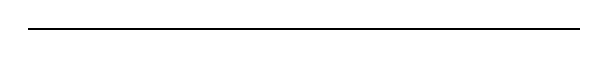
\begin{tikzpicture}
        \draw[fill=white] (-3.5, -0.01) rectangle (3.5, 0.01);
    \end{tikzpicture}
    \\[4pt]
    \titlefont{Backend Developer -- Java \& Spring Boot}
}

% -- Sidebox
\posterbox[
    colback=minimal-light,
    valign=top,
    top=\inboxspacing,
    halign=right,
    right=\inboxspacing]
    {name=sidebar,
    below=headbox,
    column=1,
    span=\sideboxwidth,
    rowspan=\mainboxheight}
{
    \begin{tabular}{rl}
        & \titlefont{Contacto} \\
        \hline \mediumspace

        \multirow{2}{*}{\scalebox{0.075}{\input{icons/address.tex}}}
            & \textbf{Direcci\'{o}n} \\
                & Quito, Ecuador \\
                & \smallspace

        \multirow{2}{*}{\scalebox{0.075}{\input{icons/phone.tex}}}
            & \textbf{Tel\'{e}fono} \\
                & \href{tel:+593978729018}{(+593) 97 872 9048} \\
                & \smallspace

        \multirow{2}{*}{\scalebox{0.075}{\input{icons/email.tex}}}
            & \textbf{Correo} \\
                & \href{mailto:sdcastillo.dev@gmail.com}{sdcastillo.dev@gmail.com} \\
                & \largespace

        & \titlefont{Plataformas} \\
        \hline \mediumspace

        \multirow{2}{*}{\scalebox{0.075}{\input{icons/github.tex}}}
        & \textbf{GitHub} \\
        & \href{https://github.com/Santiago193}{github.com/Santiago193} \\
        & \smallspace

        \multirow{2}{*}{\scalebox{0.075}{\input{icons/linkedin.tex}}}
        & \textbf{LinkedIn} \\
        & \href{https://www.linkedin.com/in/sdcastillo}{linkedin.com/in/sdcastillo} \\
        & \largespace

        & \titlefont{Documentos} \\
        \hline \mediumspace

        \multirow{2}{*}{\scalebox{0.075}{

\begin{tikzpicture}

    % Background
    \fill[minimal-main] (0, 0) circle (7);

    % Foundation
    \fill[minimal-contrast] (-3.2, -5.3) rectangle (3.2, -4.7);

    % Logo
% Base del certificado
\fill[minimal-white] (-3.2,-1.5) rectangle (3.2,2);

% Marco del diploma
\draw[minimal-main, line width=1pt] (-2.6,-0.8) rectangle (2.6,1.4);

% Líneas simulando texto
\fill[minimal-main] (-2.2,0.9) rectangle (2.2,1.1);
\fill[minimal-main] (-2.2,0.4) rectangle (1.8,0.6);
\fill[minimal-main] (-2.2,0.0) rectangle (2.0,0.2);

% Sello circular
\draw[minimal-main, line width=1pt] (1.8,-0.3) circle (0.4);

% Cintas del sello
\fill[minimal-main] (1.6,-0.7) -- (1.8,-0.4) -- (2.0,-0.7) -- cycle;
\fill[minimal-main] (1.7,-0.9) -- (1.8,-0.5) -- (1.9,-0.9) -- cycle;


\end{tikzpicture}}}
        & \textbf{Certificaciones y Premios} \\
        & \href{https://drive.google.com/drive/folders/1T03rp3wPN2O0gNA2CDsZuldCbB4yA8ph?usp=sharing}
        {\fcolorbox{minimal-main}{minimal-contrast}{\small\textbf{ Ver carpeta en Drive }}} \\
        & \largespace

        & \titlefont{Referencias} \\
        \hline \mediumspace

        \multirow{2}{*}{\scalebox{0.075}{
\begin{tikzpicture}

    % Background
    \fill[minimal-main] (0, 0) circle (7);

% Cabeza
\fill[minimal-white] (0,2.2) circle (1.2);

% Hombros más estrechos y naturales
\fill[minimal-white]
(-2.6,-3)
.. controls (-2.6,-0.8) and (-1.4,0.3) .. (0,0.3)
.. controls (1.4,0.3) and (2.6,-0.8) .. (2.6,-3)
-- cycle;2.5,0.5) and (4,-0.5) .. (4,-3)
-- cycle;
    
\end{tikzpicture}}}
            & \textbf{Rodrigo E. Tufino} \\
            & Docente UPS \\
            & \href{mailto:rtufino@ups.edu.ec}{rtufino@ups.edu.ec} \\
            & \smallspace

        \multirow{4}{*}{\scalebox{0.075}{
\begin{tikzpicture}

    % Background
    \fill[minimal-main] (0, 0) circle (7);

% Cabeza
\fill[minimal-white] (0,2.2) circle (1.2);

% Hombros más estrechos y naturales
\fill[minimal-white]
(-2.6,-3)
.. controls (-2.6,-0.8) and (-1.4,0.3) .. (0,0.3)
.. controls (1.4,0.3) and (2.6,-0.8) .. (2.6,-3)
-- cycle;2.5,0.5) and (4,-0.5) .. (4,-3)
-- cycle;
    
\end{tikzpicture}}}
            & \textbf{Ing. Daniel Diaz, MSc.} \\
            & Director de carrera \\
            & Ing. en Computaci\'{o}n \\
            & \href{tel:+593997656412}{(+593) 99 765 6412} \\
            & \href{mailto:ddiaz@ups.edu.ec}{ddiaz@ups.edu.ec} \\
            & \largespace

        & \titlefont{Idiomas} \\
        \hline \mediumspace

        \multirow{2}{*}{\scalebox{0.075}{
\begin{tikzpicture}

    % Clip circular
    \clip (0,0) circle (7);

    % Franja superior roja
    \fill[red] (-7,2.33) rectangle (7,7);

    % Franja central amarilla
    \fill[yellow] (-7,-2.33) rectangle (7,2.33);

    % Franja inferior roja
    \fill[red] (-7,-7) rectangle (7,-2.33);

\end{tikzpicture}}}
            & \textbf{Espa\~{n}ol} \\
            & Nativo \\
            & \smallspace

        \multirow{2}{*}{\scalebox{0.075}{\input{flags/britain.tex}}}
            & \textbf{Ingl\'{e}s} \\
            & B2 \\
            & \smallspace

    \end{tabular}
}

% -- Mainbox
\posterbox[
    colback=white,
    valign=top,
    top=\inboxspacing,
    halign=left,
    left=\inboxspacing]
    {name=mainbox,
    column*=1,
    span=\mainboxwidth,
    below=headbox,
    rowspan=\mainboxheight}
{
\begin{tabularx}{\linewidth}{>{\footnotesize}r X}
    & \titlefont{Perfil Profesional} \\
    \hline \mediumspace

\multicolumn{2}{p{\linewidth}}{
Desarrollador Backend especializado en Java 11 y Java 21 con Spring Boot 3, con experiencia construyendo APIs RESTful seguras con autenticaci\'{o}n JWT, autorizaci\'{o}n basada en roles y persistencia en PostgreSQL. Familiarizado con despliegue en entornos Linux usando Docker y Nginx, y con el ciclo completo de desarrollo desde el dise\~{n}o de la API hasta la puesta en producci\'{o}n.
} \\

    \largespace
    & \titlefont{Educaci\'{o}n} \\
    \hline \mediumspace

    Oct 2023 -- Presente
        & \textbf{Universidad Polit\'{e}cnica Salesiana} \\
        & Ingenier\'{i}a en Ciencias de la Computaci\'{o}n \\
        & Sexto Semestre \\
        & Promedio: 90.97 / 100 \\
        & \smallspace

    Sep 2010 -- Jul 2023
        & \textbf{Unidad Educativa Paulo VI} (Bachillerato) \\
        & Promedio: 9.69 / 10 \\

\end{tabularx}

\largespace

\begin{tabularx}{\linewidth}{>{\footnotesize\raggedleft}p{0.8cm} X}

    & \titlefont{Logros y Premios} \\
    \hline \mediumspace

    2026
        & \textbf{1er Lugar -- Proyecto Integrador UPS -- MotoSOS} \\
        & \href{https://drive.google.com/file/d/1rqDxcfqPQAIeVpiW-KUCwLK33JLMLdo8/view?usp=sharing}{Ver certificado} \\
        & \smallspace

    2025
        & \textbf{3er Lugar -- CTF Internacional (UPS)} \\
        & \href{https://www.instagram.com/p/DRfCaPtkZOV}{Ver publicaci\'{o}n} \; | \;
          \href{https://drive.google.com/file/d/1jrjPrLftk4szXN4mIPCdAZkPwd03pHbe/view?usp=sharing}{Ver certificado} \\
        & \smallspace

    2025
        & \textbf{1er Lugar -- Cisco Topology War} \\
        & \href{https://www.linkedin.com/posts/sdcastillo_ciscotopologywar-cisco-networking-activity-7409019921684246528-kXen}{Ver publicaci\'{o}n} \\
        & \smallspace

    2025
        & \textbf{3er Lugar -- Competencia de Programaci\'{o}n en Java} \\
        & \href{https://drive.google.com/file/d/1Dc9aeAVjurLVU1okpf_xe2OyIYzcQzAi/view}{Ver certificado} \\
        & \smallspace

    2025
        & \textbf{3er Lugar -- Hackathon ``Innovando por Esmeraldas''} \\
        & \href{https://www.instagram.com/p/DI_xq1CzpiY/}{Ver publicaci\'{o}n} \\
        & \smallspace

\end{tabularx}

\largespace

\begin{tabularx}{\linewidth}{>{\footnotesize\raggedleft}p{1.6cm} X}

    & \titlefont{Habilidades T\'{e}cnicas} \\
    \hline \mediumspace

    \textbf{Dominio}
        & Java 21, Spring Boot 3, Spring Security, JWT, APIs REST, Spring MVC, JDBC, JPA, JSP, Servlets \\
        & \smallspace

    \textbf{BD}
        & PostgreSQL, MySQL \\
        & \smallspace

    \textbf{Servidores}
        & Apache Tomcat, WildFly \\
        & \smallspace

    \textbf{DevOps}
        & Linux, Docker, Nginx, Git, Maven \\
        & \smallspace

    \textbf{Frontend}
        & Angular, TailwindCSS \\
        & \smallspace

    \textbf{Otros}
        & Bash, ESP32, n8n \\

\end{tabularx}
}

% -- Footbox
\posterbox[colback=minimal-main]
           {name=blankbox2,
           below=sidebar,
           column=1,
           span=1,
           rowspan=\footboxheight}{}

\end{tcbposter}

% =====================================================================
% PAGINA 2
% =====================================================================
\newpage

\begin{tcbposter}[
    poster = {columns=1, rows=1, spacing=0pt},
    boxes = {sharp corners, halign=center, valign=center, boxrule=0pt}
]

% ---------------- MAINBOX ----------------
\posterbox[
    colback=white,
    valign=top,
    top=\inboxspacing,
    halign=left,
    left=\inboxspacing]
    {name=mainbox,
    column=1,
    span=1,
    rowspan=\mainboxheight}
{

\begin{tabularx}{\linewidth}{X}

\titlefont{EXPERIENCIA} \\
\hline \mediumspace

{\large\textbf{\color{minimal-black}Pr\'{a}cticas Profesionales -- nDeveloper}} \hfill
\textbf{Abr 2026 -- Jul 2026} \quad
\fcolorbox{minimal-green}{white}{\small\textbf{\color{minimal-green}$\bullet$ En curso}} \\

Desarrollo en equipo sobre una plataforma SaaS multitenant para el sector salud, sirviendo m\'{u}ltiples empresas desde una sola instancia. Implementaci\'{o}n de m\'{o}dulos de gesti\'{o}n de sucursales y selecci\'{o}n de m\'{e}dico por especialidad en Angular, correcci\'{o}n de incidencias y mantenimiento del backend Java 11 desplegado en WildFly. \\
\textbf{Tecnolog\'{i}as:} Java 11, WildFly, Angular 17, Arquitectura Multitenant. \\

\end{tabularx}

\largespace
\largespace

\begin{tabularx}{\linewidth}{X}

\titlefont{PROYECTOS} \\
\hline \mediumspace

{\large\textbf{\color{minimal-black}Tienda -- Sistema POS y Facturaci\'{o}n}} \hfill
\textbf{2026 -- Presente} \quad
\fcolorbox{minimal-green}{white}{\small\textbf{\color{minimal-green}$\bullet$ En Desarrollo}} \\

API REST con Spring Boot 3 para sistema POS: autenticaci\'{o}n JWT con roles diferenciados (Administrador / Empleado), dise\~{n}o de esquema PostgreSQL normalizado, arquitectura en capas (Controller -- Service -- Repository) y frontend desacoplado en Angular 19. Integraci\'{o}n planificada con facturaci\'{o}n electr\'{o}nica SRI. \\
\textbf{Tecnolog\'{i}as:} Java 21, Spring Boot 3, Spring Security, JWT, PostgreSQL, Angular 19, TailwindCSS 4, Maven, Apache Tomcat. \\
\textit{Repositorios: }
\href{https://github.com/Santiago193/1016-scastillo-app-java-spring-facturas-pos-backend}{tienda-backend}
\; | \;
\href{https://github.com/Santiago193/1016-scastillo-app-angular-facturas-pos-frontend}{tienda-frontend}

\\[10pt]

{\large\textbf{\color{minimal-black}MotoSOS -- Sistema de Detecci\'{o}n y Alerta de Accidentes}}
\hfill \textbf{2026} \\

Sistema de alertas en tiempo real ante accidentes de moto: detecci\'{o}n por fusi\'{o}n de sensores, confirmaci\'{o}n para descartar falsas alarmas y notificaci\'{o}n autom\'{a}tica v\'{i}a Telegram API y dashboard Angular. 1er lugar Proyecto Integrador UPS. \\
\textbf{Tecnolog\'{i}as:} Node.js, WebSockets, Telegram API, Angular, ESP32.

\end{tabularx}
}

\posterbox[colback=minimal-main]
{name=blankbox2,
below=sidebar,
column=1,
span=1,
rowspan=\footboxheight}{}

\end{tcbposter}

\end{document}
